\section{$\Km$-$\pip$ Detection Asymmetry}
\label{sec:KpiAsym}

The presented measurement of the CKM-angle $\gamma$ using $\Bs\to\Ds\kaon\pion\pion$ decays is sensitive to a possible charge asymmetry of the kaon. 
This effect can be detector induced, because kaons are known to have a nuclear cross-section which is asymmetrically dependent on the sign of their charge. 
It is indispensable to determine the detector induced charge asymmetry of the kaon, as fitting without taking this effect into account would introduce a 'fake' CP violation. \newline

Instead of determining the single track detection asymmetry of a kaon, it is found \cite{Gordon:1482647} that the combined two track asymmetry of a kaon-pion pair is much easier to access. 
Therefore the two track asymmetry is used, which is definded as 
   

\begin{equation}
A^{det}(\Km\pip) = \frac{\epsilon^{det}(\Km\pip) -\epsilon^{det}(\Kp\pim)}{\epsilon^{det}(\Km\pip) + \epsilon^{det}(\Kp\pim)}.
\label{eq:KpiDetAsymDef}
\end{equation}


$A^{det}(\Km\pip$ can further be expressed, assuming no CP violation in Cabbibo-favoured charm modes, as \cite{Davis:2310213}

\begin{equation}
\begin{split}
A^{det}(\Km\pip) = & \frac{N(\Dp\to\Km\pip\pip) - N(\Dm\to\Kp\pim\pim)}{N(\Dp\to\Km\pip\pip) + N(\Dm\to\Kp\pim\pim)} \\
                  & - \frac{N(\Dp\to\KS\pip) - N(\Dm\to\KS\pim)}{N(\Dp\to\KS\pip) + N(\Dm\to\KS\pim)} \\
                  & - A(\Kz),
\end{split}
\label{eq:KpiDetAsymDef}
\end{equation}

where possible CP violation in the $\Dp\to\KS\pip$ mode is predicted to be smaller than $10^{-4}$ in the Standard Model \cite{Bigi:1994aw}.
Using Eq. \ref{eq:KpiDetAsymDef}, the two track $\Km$-$\pip$ asymmetry is obtained from the difference in asymmetries in the $\Dp\to\Km\pip\pip$ and $\Dp\to\KS\pip$ modes. 
$A(\Kz)$ is the asymmetry in the neutral kaon system and has to be taken into account as a correction. \newline

We use a dedicated LHCb tool to determine $A^{det}(\Km\pip)$ for all data taking periods used in this analysis. A detailed description, along with all plots ca be found in \cite{Davis:2310213}.
The tool provides large calibration samples of $\Dpm\to\Kpm\pipm\pipm$ and $\Dpm\to\KS\pipm$ decays, which are used to determine the asymmetry following Eq. \ref{eq:KpiDetAsymDef}. 
Several weighting steps are performed to match the kinematics of the calibration samples to our signal decay sample: \newline
First, weights are assigned to the $\Kpm$ and $\pipm$ of the $\Dpm\to\Kpm\pipm\pipm$ sample, using $\ptot$, $\eta$ of the $\Kpm$ and $\pt$, $\eta$ of the $\pipm$ from our $\Bs\to\Ds\kaon\pion\pion$ signal decay.
Then, weights are assigned to the $\Dpm$ ($\pt, \eta$) and the $\pipm$ ($\pt$) of the $\Dpm\to\KS\pipm$ sample to match the corresponding, weighted distributions of the $\Dpm\to\Kpm\pipm\pipm$ sample.
In a last step, weights are assigned to match the bachelor pions $\phi$ distributions between the two calibration samples. \newline
After the samples are correctly weighted, fits are performed to the invariant $m(\Km\pip\pip)$/$m(\Kp\pim\pim)$ and $m(\KS\pip)$/$m(\KS\pim)$ distributions to determine $A^{det}(\Km\pip)$. 
The PDFs used to describe the invariant mass distributions consist of gaussian functions for the signal component and exponentials describing the residual background.
The detection asymmetry is determined separately for every year and (since it is a charge asymmetry effect) magnet polarity. 
Serving as an example for Run I and Run II, the fits used to determine $N(\Dp\to\Km\pip\pip)$/$N(\Dm\to\Kp\pim\pim)$ and $N(\Dp\to\KS\pip)$/$N(\Dm\to\KS\pim)$ 
for 2011, magnet up data and 2015, magnet up data are shown in Figure \ref{fig:KpiAsymFitsRun1} and \ref{fig:KpiAsymFitsRun2} respectively.



\begin{figure}[h]
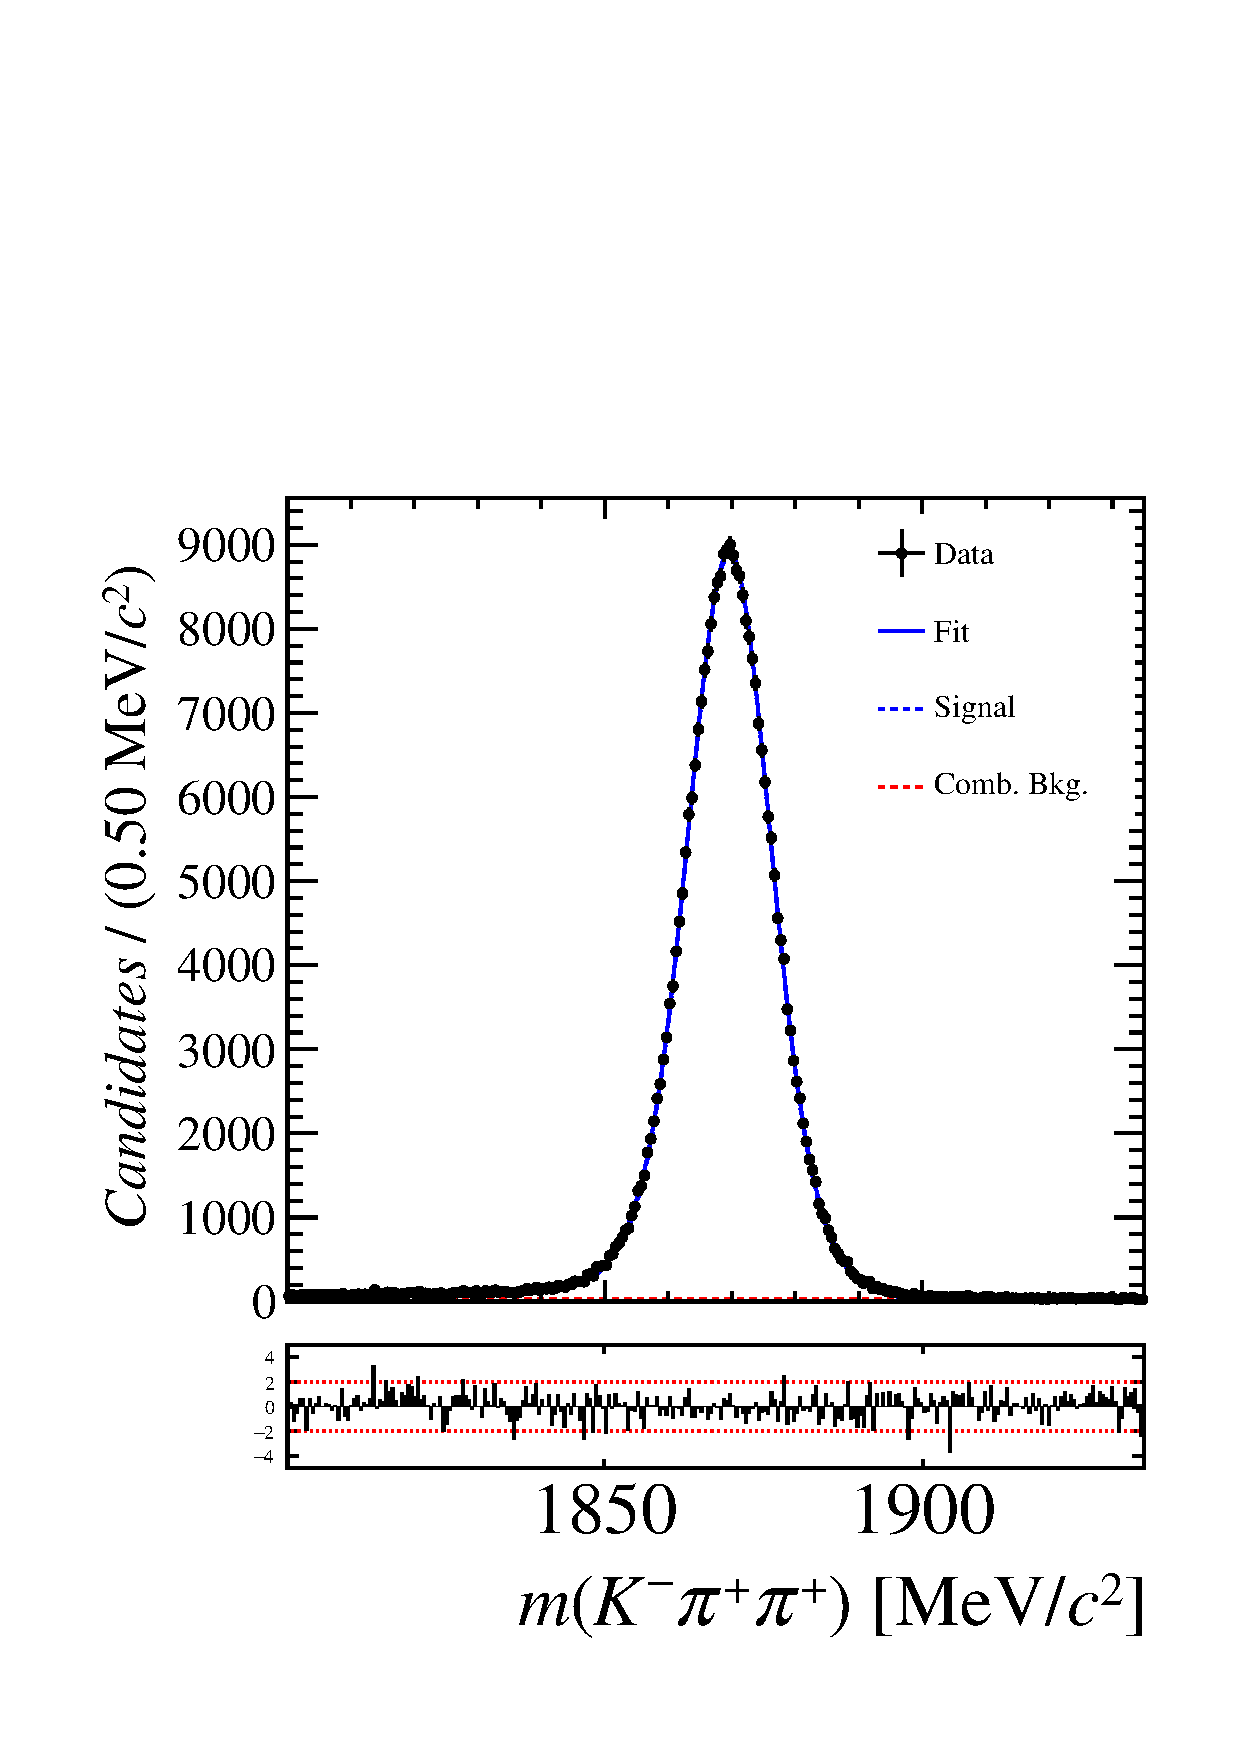
\includegraphics[height=!,width=0.4\textwidth]{figs/KpiAsym/fit_negative_kpipi_11up.pdf}
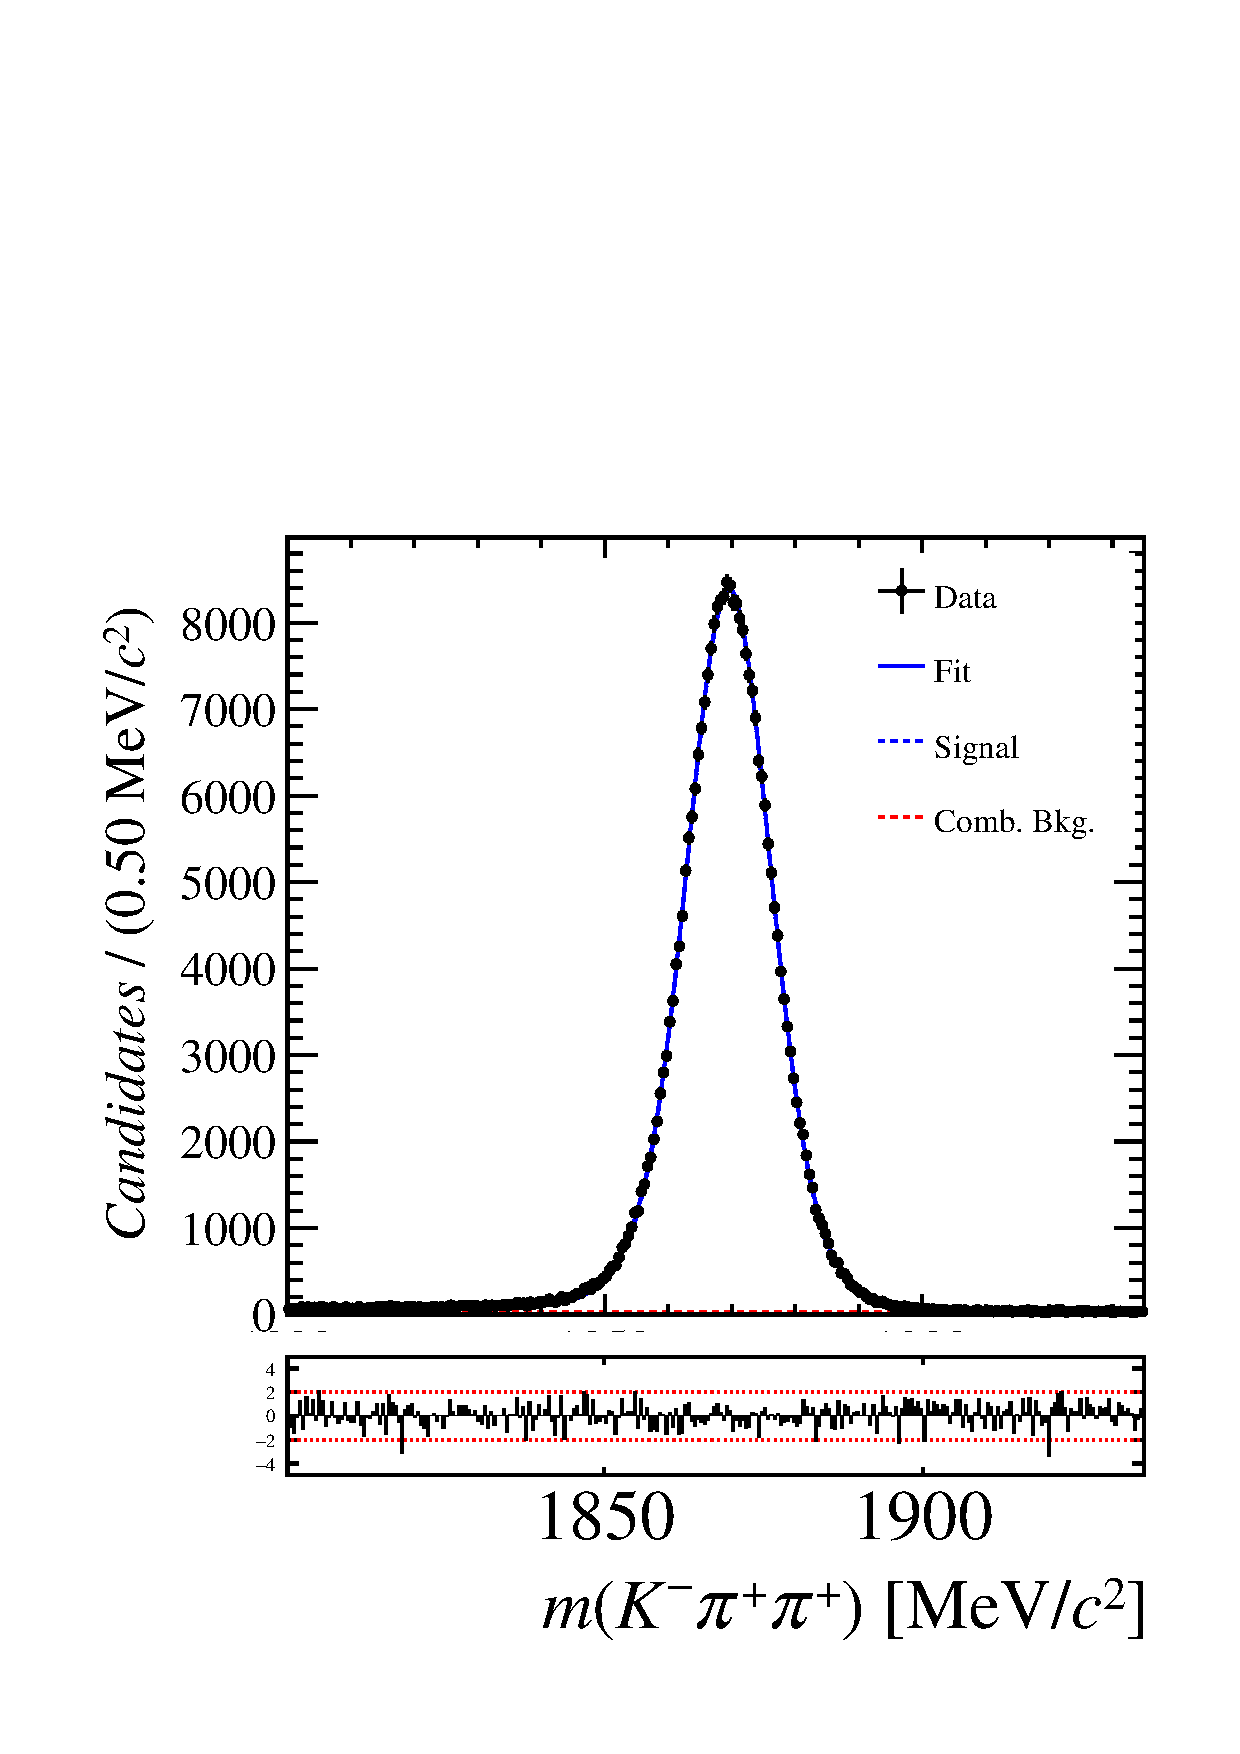
\includegraphics[height=!,width=0.4\textwidth]{figs/KpiAsym/fit_positive_kpipi_11up.pdf}\\
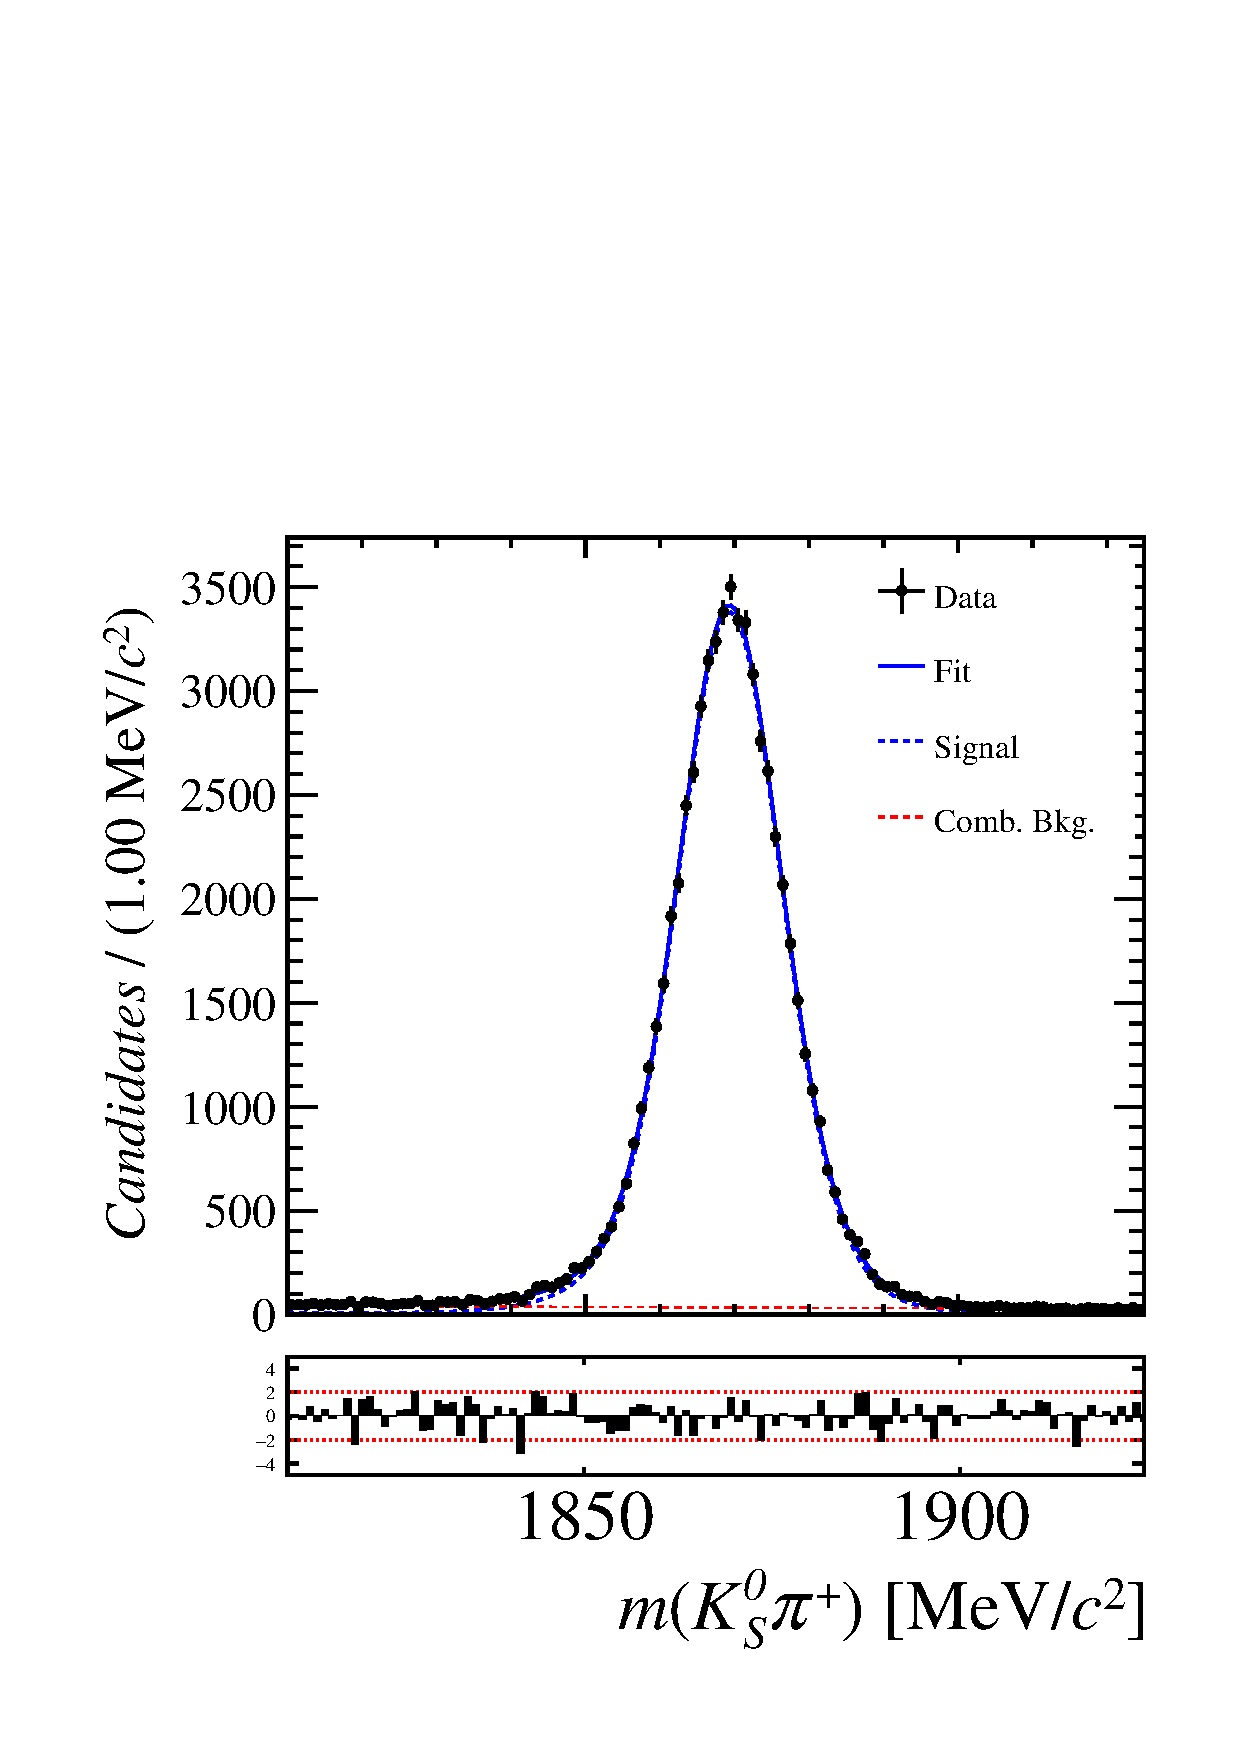
\includegraphics[height=!,width=0.4\textwidth]{figs/KpiAsym/fit_negative_kspi_11up.pdf}
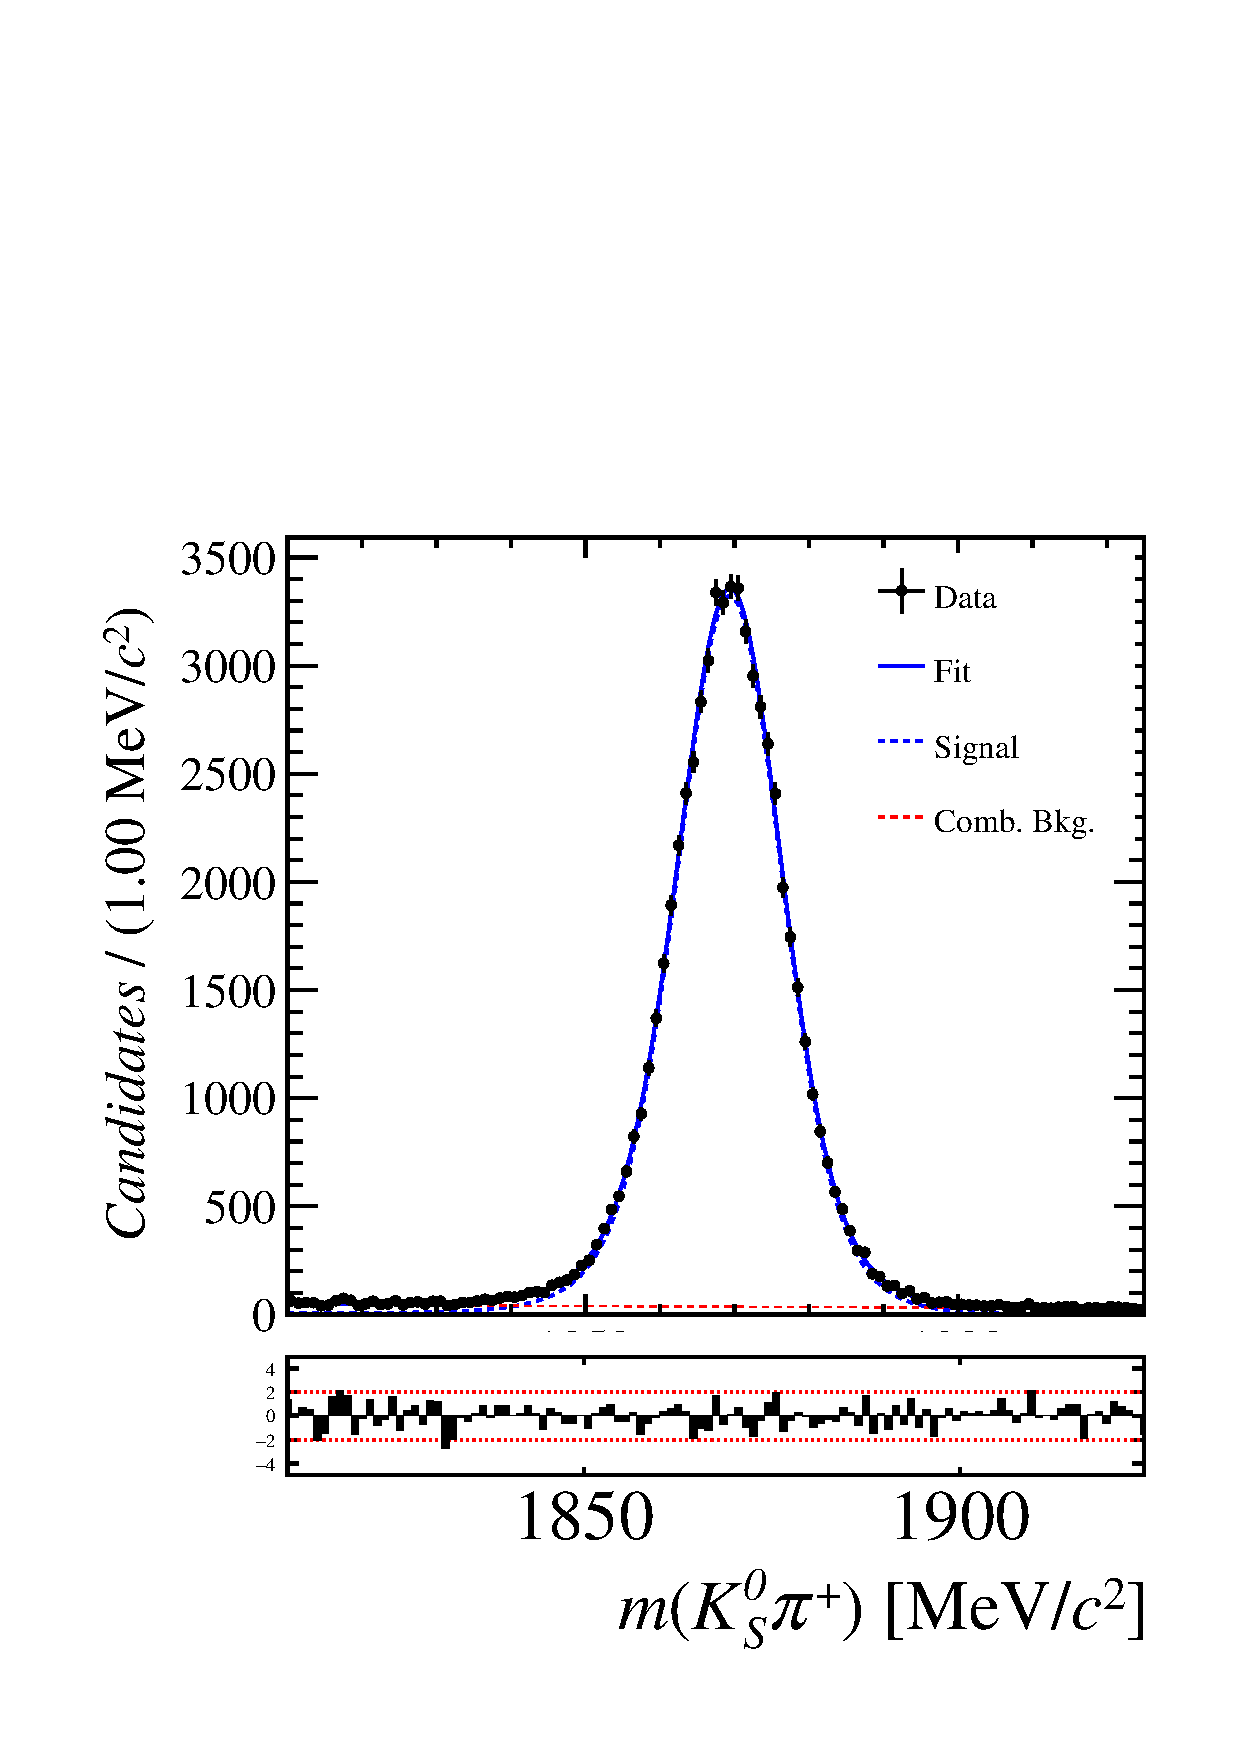
\includegraphics[height=!,width=0.4\textwidth]{figs/KpiAsym/fit_positive_kspi_11up.pdf}
\caption{Distributions of the invariant mass of (top) $\Dpm\to\Kpm\pipm\pipm$ and (bottom) $\Dpm\to\KS\pipm$ candidates for Run I data from the calibration samples. A fit described in the text is overlaid.}
\label{fig:KpiAsymFitsRun1}
\end{figure}


\begin{figure}[h]
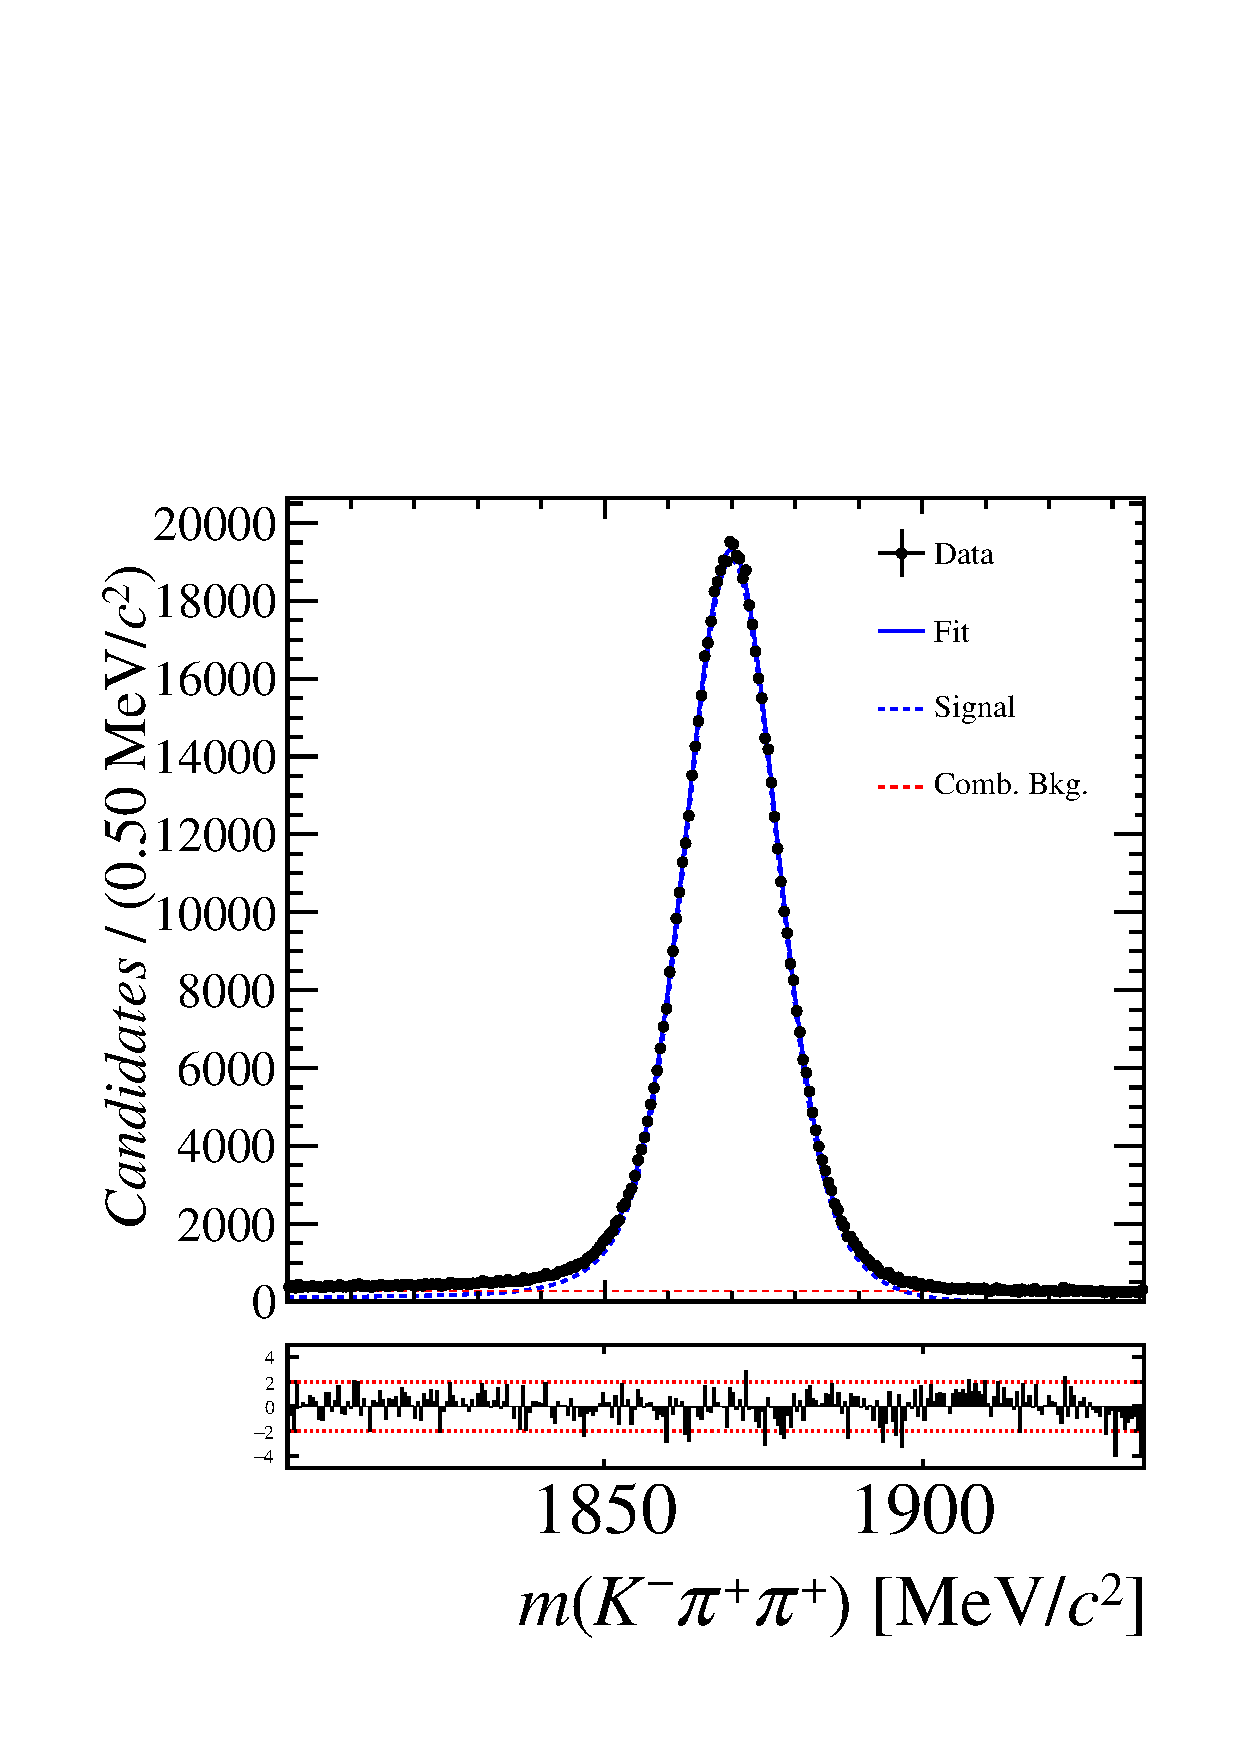
\includegraphics[height=!,width=0.4\textwidth]{figs/KpiAsym/fit_negative_kpipi_15up.pdf}
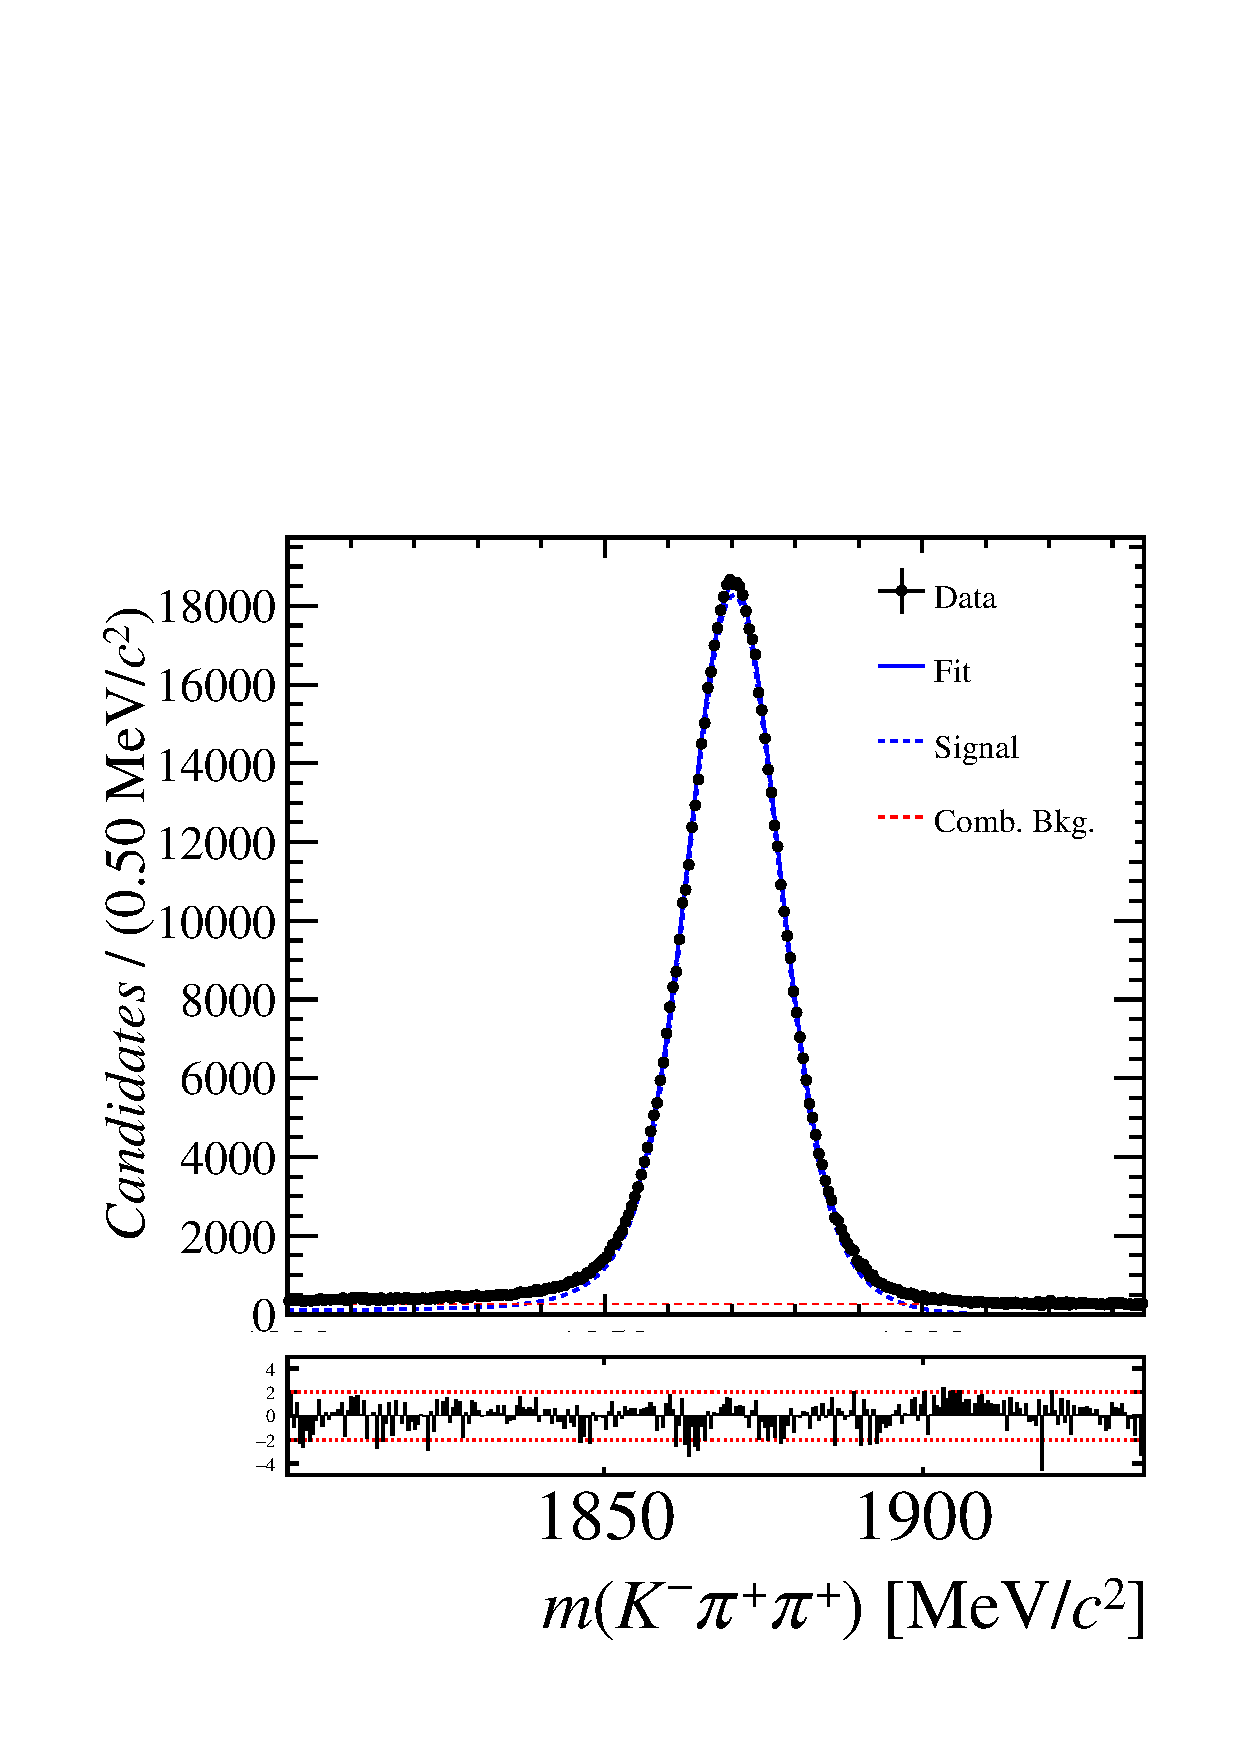
\includegraphics[height=!,width=0.4\textwidth]{figs/KpiAsym/fit_positive_kpipi_15up.pdf}\\
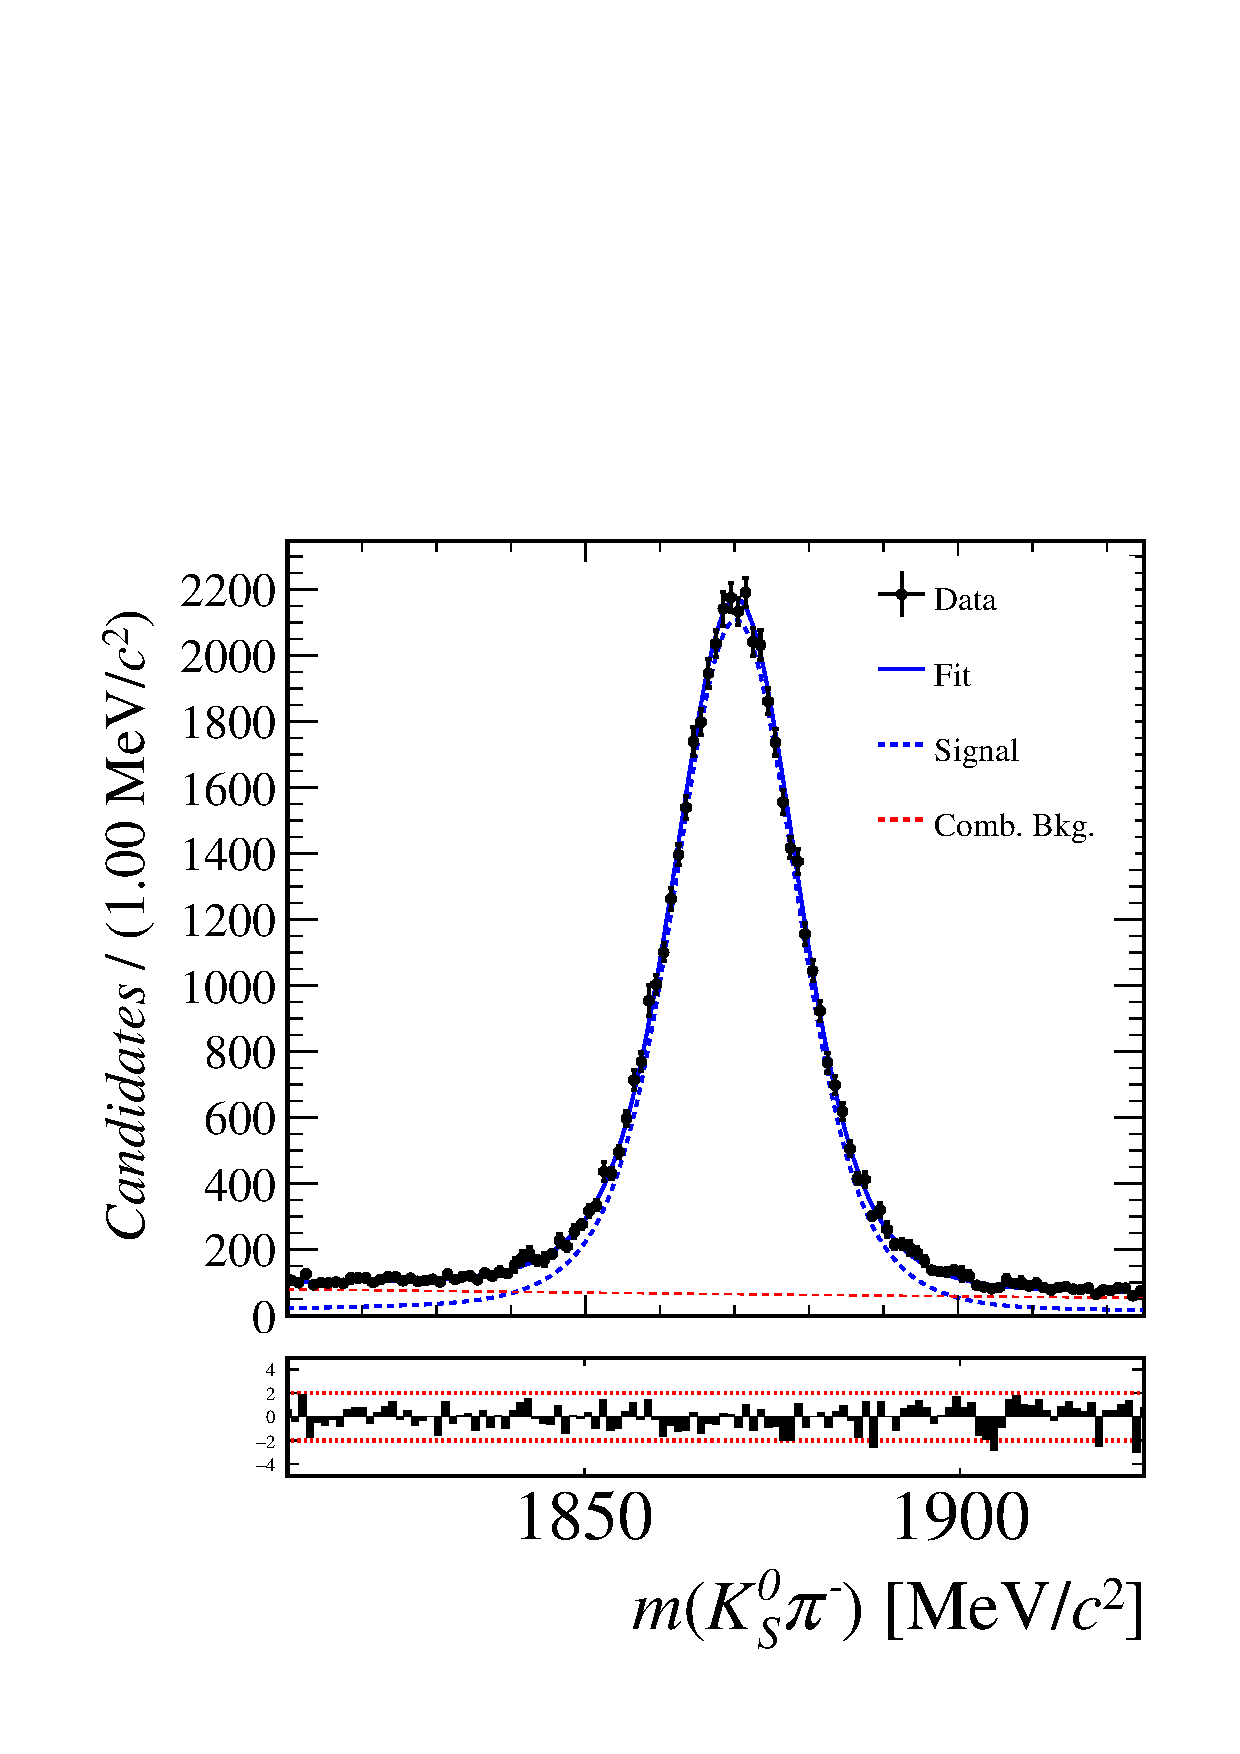
\includegraphics[height=!,width=0.4\textwidth]{figs/KpiAsym/fit_negative_kspi_15up.pdf}
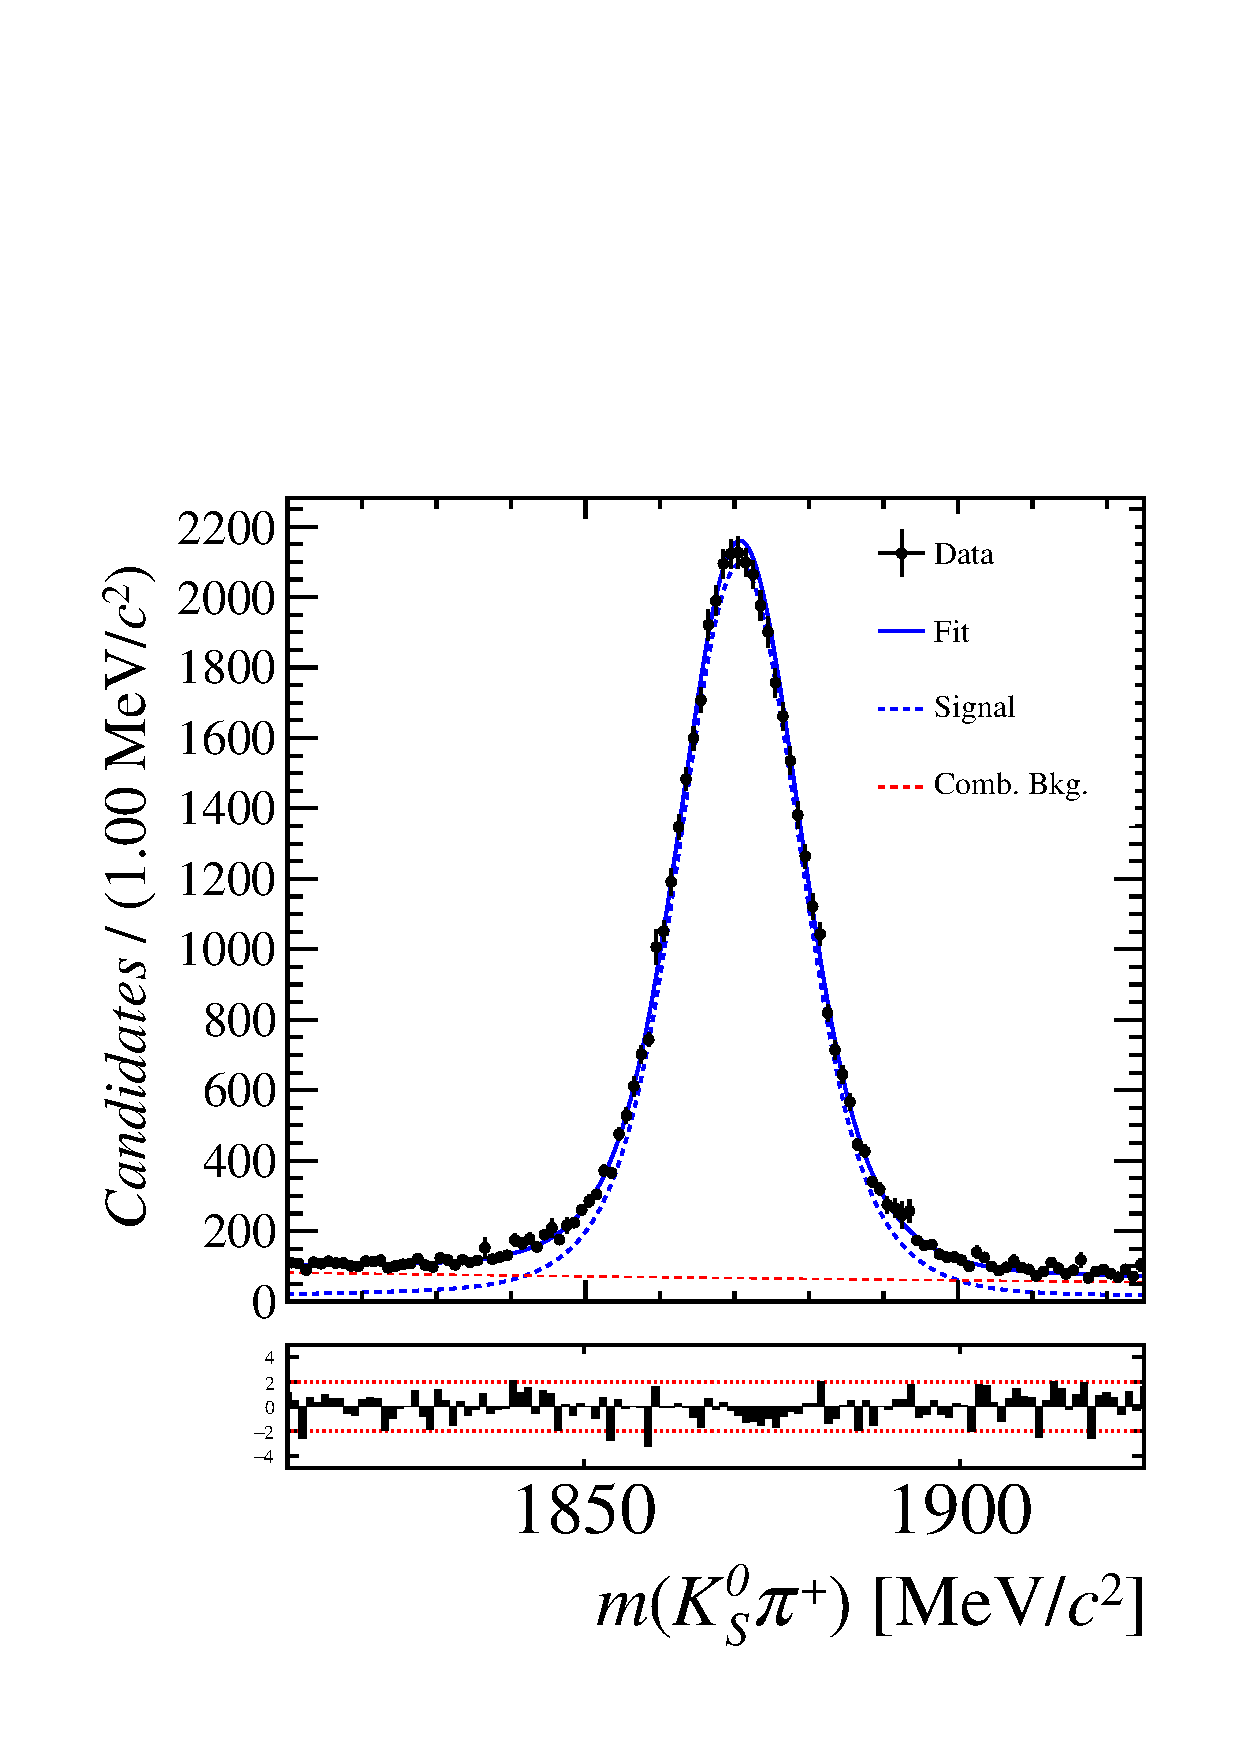
\includegraphics[height=!,width=0.4\textwidth]{figs/KpiAsym/fit_positive_kspi_15up.pdf}
\caption{Distributions of the invariant mass of (top) $\Dpm\to\Kpm\pipm\pipm$ and (bottom) $\Dpm\to\KS\pipm$ candidates for Run 2 data from the calibration samples. A fit described in the text is overlaid.}
\label{fig:KpiAsymFitsRun2}
\end{figure}


The obtained values of $A^{det}(\Km\pip)$ + $A(\Kz)$ for all years and polarities are shown in Table \ref{table:KpiDetectionAsym}.

\begin{table}[h]
\centering
 \begin{tabular}{l | l}
Data sample & $A^{det}(\Km\pip)$ + $A(\Kz)$ [\%] \\
\hline\hline
Run I & \\
\hline
2011, mag. up & -2.01 $\pm$ 0.32\\
2011, mag. down &  -0.16 $\pm$  0.28\\
2011, average & -1.09 $\pm$ 0.21\\
\hline
2012, mag. up &  -0.90 $\pm$ 0.20\\
2012, mag. down & -1.01 $\pm$ 0.22 \\
2012, average & -0.96 $\pm$ 0.15\\
\hline\hline
Run II &  \\
\hline
2015, mag. up & -1.36 $\pm$ 0.36 \\
2015, mag. down & -0.96 $\pm$ 0.24 \\
2015, average & -1.16 $\pm$ 0.22\\
\hline
2016, mag. up &  0.50 $\pm$ 0.88\\
2016, mag. down & 1.23 $\pm$ 0.72 \\
2016, average & 0.87 $\pm$ 0.57\\
\hline
\end{tabular}
\caption{Summary of the $\Km$-$\pip$ detection asymmetry obtained from the fits to the Run1 and Run2 calibration samples.}
\label{table:KpiDetectionAsym}
\end{table}
